% =============================================================================
%  Project Proposal -- OS-Buddy
%  Cover and design follow the "Cubicle - Project Report" (plain
%  black headings, grey-header tables, DIU cover page). Font: Onest.
%  Build:  xelatex proposal.tex   (run twice so cross-references resolve)
%  Edit the "Project details" and "Team" blocks below; everything else follows.
% =============================================================================
\documentclass[11pt,a4paper]{article}

% ---------- Font: Onest for everything (text, code, e-mails) -----------------
% Onest has no italic, so italic text is the upright font slanted.
% The font files and their licence (SIL OFL) are in the fonts/ folder.
\usepackage{fontspec}
\setmainfont{Onest-400}[
  Path=fonts/, Extension=.ttf, Ligatures=TeX,
  UprightFont=Onest-400, BoldFont=Onest-700,
  ItalicFont=Onest-400, ItalicFeatures={FakeSlant=0.18},
  BoldItalicFont=Onest-700, BoldItalicFeatures={FakeSlant=0.18}]
\setsansfont{Onest-400}[Path=fonts/, Extension=.ttf, BoldFont=Onest-700]
\setmonofont{Onest-400}[Path=fonts/, Extension=.ttf, BoldFont=Onest-700]

% ---------- Layout ----------------------------------------------------------
\usepackage[a4paper,top=2.5cm,bottom=2.2cm,left=2.5cm,right=2.5cm,nohead]{geometry}
\usepackage{graphicx}
\usepackage{xcolor}
\usepackage{array}
\usepackage{tabularx}
\usepackage{caption}
\usepackage{float}                  % [H]: keep each table where it is written
\usepackage[hidelinks]{hyperref}
\usepackage{tikz}                   % use case and sequence diagrams
\usetikzlibrary{arrows.meta,shapes.geometric}

% ---------- Project details (edit these) ------------------------------------
\newcommand{\projectname}{OS-Buddy}
\newcommand{\projectsubtitle}{An Agentic Operating-System Operator in Bash,\\ Designed with the PEAS Model}
\newcommand{\coursecode}{CSE324}
\newcommand{\coursetitle}{Operating Systems Lab}
\newcommand{\proposaldate}{13 November 2026}

% ---------- Team (edit names, IDs, e-mails) ---------------------------------
\newcommand{\memA}{Mst. Washima Zinat Snigdha}
\newcommand{\memB}{Umma Iman Monea}
\newcommand{\memC}{Md. Kawsar Ahamed}
\newcommand{\memD}{Md Himel Ahmed}
\newcommand{\memE}{Shagato Chowdhury}

\hypersetup{pdftitle={OS-Buddy: Project Proposal},pdfsubject={Group project proposal},
  pdfkeywords={agentic AI, Bash, Gemini, PEAS, operating system}}

% ---------- Look and feel (matches the report) ------------------------------
\setlength{\parindent}{0pt}                  % left-aligned text, a small gap between paragraphs
\setlength{\parskip}{3pt}
\renewcommand{\arraystretch}{1.3}          % taller table rows
\setlength{\tabcolsep}{7pt}                   % more space left and right inside cells
\definecolor{hdrgrey}{gray}{0.90}
\newcommand{\code}[1]{#1}     % same font as the text
\captionsetup{font=small,labelfont=bf,skip=4pt}

\makeatletter
\renewcommand\section{\@startsection{section}{1}{\z@}%
  {1.6ex \@plus .4ex \@minus .2ex}{0.8ex \@plus .2ex}{\normalfont\large\bfseries}}
\renewcommand\subsection{\@startsection{subsection}{2}{\z@}%
  {1.2ex \@plus .3ex \@minus .2ex}{0.5ex \@plus .2ex}{\normalfont\normalsize\bfseries}}
\makeatother

\pagestyle{empty}                % no header, no page number

% Grey table header and compact lists
% The grey fill stops just short of each cell edge, so the vertical borders stay visible.
\newcommand{\hdrrow}{\rowcolor{hdrgrey}[\dimexpr\tabcolsep-0.4pt\relax][\dimexpr\tabcolsep-0.4pt\relax]}
\usepackage{colortbl}
\newcommand{\tightlist}{\setlength{\itemsep}{0pt}\setlength{\parsep}{0pt}\setlength{\topsep}{2pt}\setlength{\parskip}{0pt}}
\newcommand{\lead}[1]{\textbf{#1}}
\newcolumntype{R}[1]{>{\raggedright\arraybackslash}p{#1}}
\newcolumntype{Y}{>{\raggedright\arraybackslash}X}     % flexible column, left-aligned

\setcounter{secnumdepth}{0}      % headings have no numbers
\begin{document}
\raggedright

% =============================================================================
%  COVER PAGE
% =============================================================================
\thispagestyle{empty}
\begin{center}
  \vspace*{1.6cm}
  
\includegraphics[width=0.52\textwidth]{diu-logo.png}\\[1.0em]
  {\bfseries Faculty of Science and Information Technology}\\
  Department of Computer Science and Engineering\\[2.4em]
  \rule{\linewidth}{0.5pt}\\[2.2em]
  {\fontsize{40}{44}\selectfont\bfseries \projectname}\\[0.6em]
  {\Large \projectsubtitle}\\[2.2em]
  \rule{\linewidth}{0.5pt}\\[2.2em]
  {\small A project proposal submitted for \quad \textbf{\coursecode\ \textbar\ \coursetitle}}\\[1.4em]

  {\small\bfseries SUBMITTED BY}\\[0.3em]
  \begingroup\small
  \begin{tabular}{|R{4.9cm}|R{2.3cm}|R{5.6cm}|}
    \hline
    \hdrrow \textbf{Name} & \textbf{Student ID} & \textbf{Email} \\ \hline
    \memA & 241-15-811 & {\footnotesize{zinat241-15-811@diu.edu.bd}} \\ \hline
    \memB & 241-15-540 & {\footnotesize{iman241-15-540@diu.edu.bd}} \\ \hline
    \memC & 241-15-309 & {\footnotesize{kawsar241-15-309@diu.edu.bd}} \\ \hline
    \memD & 232-15-675 & {\footnotesize{ahmed2305101675@diu.edu.bd}} \\ \hline
    \memE & 241-15-331 & {\footnotesize{shagato241-15-331@diu.edu.bd}} \\ \hline
  \end{tabular}\\[1.2em]

  {\small\bfseries SUPERVISED BY}\\[0.3em]
  \begin{tabular}{|R{14.4cm}|}
    \hline
    \hdrrow \textbf{Ms. Tamanna Sultana} \\ \hline
    Lecturer\\
    Department of Computer Science and Engineering\\
    Faculty of Science and Information Technology, Daffodil International University \\ \hline
  \end{tabular}\\[1.2em]
  \endgroup
  {\small \proposaldate}
\end{center}
\newpage
\setcounter{page}{1}

% =============================================================================
%  BODY
% =============================================================================
{\LARGE\bfseries Project Proposal}\\[-0.1em]
\rule{\linewidth}{0.8pt}\vspace{0.4em}

\section{Title}
\textbf{\projectname: An Agentic Operating-System Operator in Bash, Designed with the PEAS Model}

\section{Project Statement}
Our project is based on the following statement from the course project list.

\begin{table}[H]
\centering
\small
\begin{tabularx}{\linewidth}{|Y|}
\hline
\hdrrow \textbf{Assigned project: 9. Shell Script based Project} \\ \hline
Write shell scripts that automate various system administration tasks. These tasks include
process management, disk monitoring, backup automation, system health monitoring, and user
management. The complexity of the project can vary based on the tasks performed, ranging from
simple file handling to more advanced process and network management. \\ \hline
\end{tabularx}
\end{table}

\lead{What we plan to do:} We will write one shell script for each task in the statement. We will
also add one screen that shows everything together. To go further, we will add an AI helper that
can do other tasks when the user asks for them in plain English. Every script will show clear
results in the terminal and ask before it changes anything (Table~\ref{tab:statement}).

\begin{table}[H]
\centering
\caption{How \projectname\ will cover the project statement.}
\label{tab:statement}
\small
\begin{tabularx}{\linewidth}{|R{3.0cm}|R{3.1cm}|Y|}
\hline
\hdrrow \textbf{Task in the statement} & \textbf{Planned command} & \textbf{What it will do} \\ \hline
Process management & \code{os-buddy proc} & Show running programs, find one by name, and stop it
  after asking. \\ \hline
Disk monitoring & \code{os-buddy disk} & Show how full each disk is and warn when it is almost
  full. \\ \hline
Backup automation & \code{os-buddy backup} & Save important folders as backup files, check them,
  restore them, and run backups on a schedule. \\ \hline
System health monitoring & \code{os-buddy health}, \code{os-buddy status} & Show the CPU, memory,
  disk and uptime in one easy report with a simple verdict. \\ \hline
User management & \code{os-buddy users} & List, add, lock and remove user accounts, while
  protecting important accounts. \\ \hline
Simple files up to advanced process and network management & AI helper: \code{os-buddy "goal"} &
  Do other tasks written in plain English, such as finding files or checking running programs,
  following safety rules. \\ \hline
\end{tabularx}
\end{table}

\section{Description}
Using a Unix system means remembering many commands and knowing which ones are risky.
\lead{\projectname} will make this easier. The user will describe a goal in plain English, such
as ``find the biggest files in this folder''. The AI helper will choose the steps, carry them
out, check the results, and keep going until the goal is done, or say clearly that it could not
do it. It will be written in Bash and will use Google's Gemini AI to choose each step.

\lead{A safety layer will sit between the AI and the computer:} Safe commands that only read
information will run on their own, anything that changes something will ask the user first, and
dangerous commands will always be blocked. \projectname\ will work on Linux and similar
systems, either as a chat or as a single command for one task. The admin scripts in
Table~\ref{tab:statement} will work without any AI.

\section{Problem and Objectives}
AI tools can suggest shell commands, but running them without checking can be unsafe, and most
chat tools leave the checking to the user. This project will build a helper that completes
tasks while keeping the user in control. Our objectives are:
\begin{itemize}\tightlist
  \item an AI helper that plans a task, does it and checks the result;
  \item safety rules that decide what runs freely, what needs approval and what is blocked;
  \item simple admin scripts for the five tasks, which work without AI;
  \item a reliable connection to the Gemini AI that keeps the secret key safe;
  \item tests that show everything works on Mac and Linux.
\end{itemize}

\section{Design Approach and Scope}
We will describe the helper with the PEAS model (Table~\ref{tab:peas}), which lists what the
helper aims for, where it works, what it can do and what it can sense. The code will be split
into small parts that each do one job, so it is easy to read and change.
\emph{Out of scope:} running directly on Windows, a graphical interface, and any change made
without the user's approval.

\begin{table}[H]
\centering
\caption{PEAS summary of \projectname.}
\label{tab:peas}
\small
\begin{tabularx}{\linewidth}{@{}|>{\bfseries}p{2.2cm}|Y|@{}}
\hline
\hdrrow Component & \textbf{Specification} \\ \hline
Performance & Finish the task correctly, follow the safety rules, recover from mistakes, and stop
  after a reasonable number of steps. \\ \hline
Environment & A Linux or Unix computer, a person at the terminal, and the Gemini AI service. \\ \hline
Actuators & Run commands, read and write files, ask the user questions, and run the admin scripts,
  always through the safety rules. \\ \hline
Sensors & What commands print, file contents, facts about the computer, and the user's replies. \\ \hline
\end{tabularx}
\end{table}

\section{How the Agent Works}
Figure~\ref{fig:usecase} shows who uses \projectname\ and what they can do. The user gives a goal,
approves or denies changes, and answers questions. The Gemini AI only plans; the computer is only
touched through the safety rules. The admin scripts need neither the AI nor a network.

\begin{figure}[!t]
\centering
\resizebox{\linewidth}{!}{%
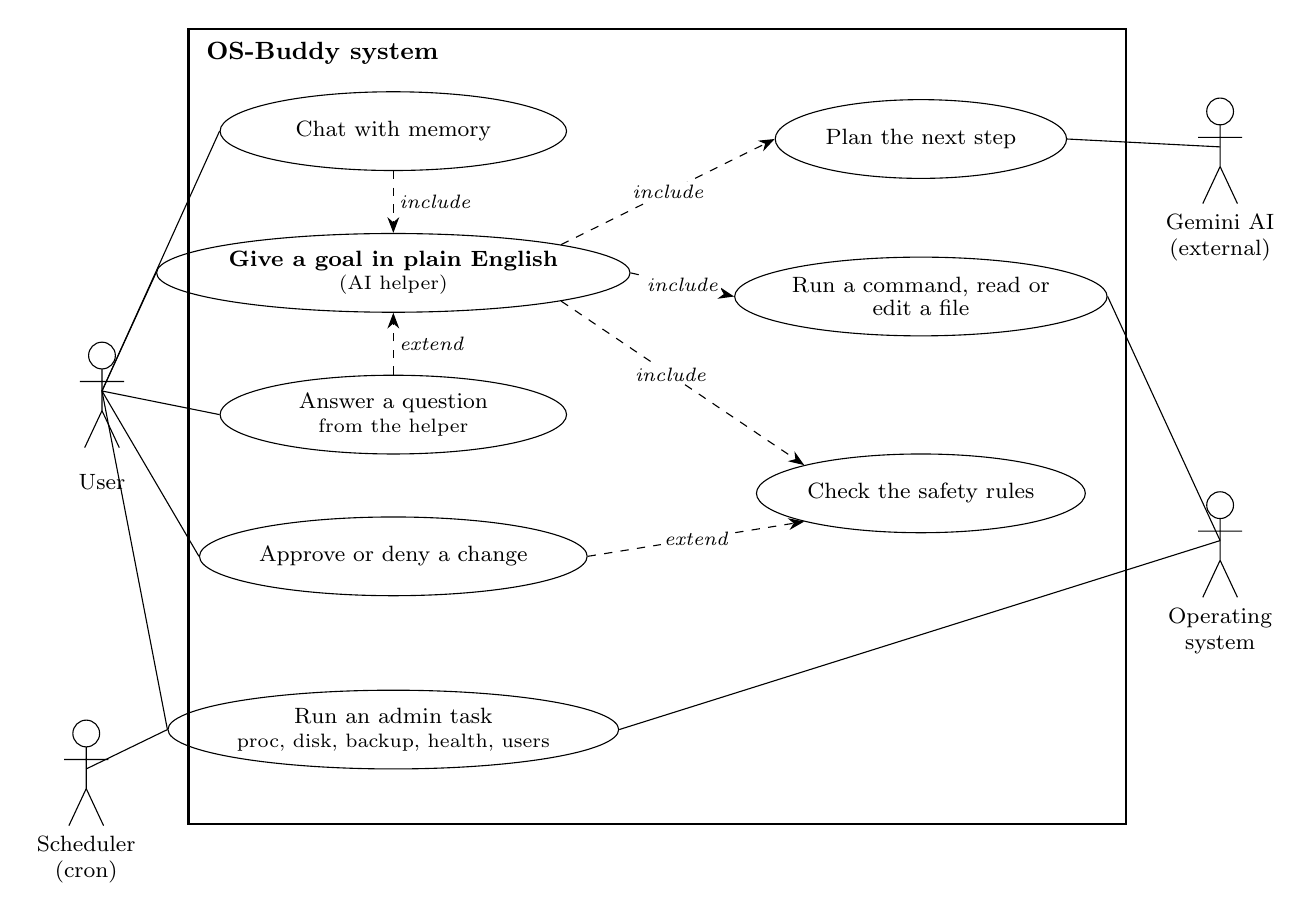
\begin{tikzpicture}[
  font=\footnotesize,
  uc/.style={ellipse,draw,align=center,inner sep=1pt,minimum height=1.0cm},
  act/.style={font=\footnotesize,align=center},
  inc/.style={-{Stealth[length=2mm]},dashed},
  lbl/.style={midway,fill=white,font=\scriptsize\itshape,inner sep=1pt}]
% stick figure at (x,y); body centre is the connection point
\newcommand{\actor}[4]{%
  \draw (#1,#2+0.55) circle (0.17);
  \draw (#1,#2+0.38) -- (#1,#2-0.15) (#1-0.28,#2+0.22) -- (#1+0.28,#2+0.22)
        (#1,#2-0.15) -- (#1-0.22,#2-0.62) (#1,#2-0.15) -- (#1+0.22,#2-0.62);
  \node[act] at (#1,#2-1.05) {#3};
  \coordinate (#4) at (#1,#2+0.1);}
% system boundary
\draw[thick] (2.0,-3.5) rectangle (13.9,6.6);
\node[anchor=north west,font=\small\bfseries] at (2.1,6.55) {\projectname\ system};
% use cases the user starts
\node[uc,minimum width=4.4cm] (chat)  at (4.6, 5.3) {Chat with memory};
\node[uc,minimum width=4.4cm] (goal)  at (4.6, 3.5) {\textbf{Give a goal in plain English}\\[-1pt]\scriptsize(AI helper)};
\node[uc,minimum width=4.4cm] (ask)   at (4.6, 1.7) {Answer a question\\[-1pt]\scriptsize from the helper};
\node[uc,minimum width=4.4cm] (appr)  at (4.6,-0.1) {Approve or deny a change};
\node[uc,minimum width=4.4cm] (admin) at (4.6,-2.3) {Run an admin task\\[-1pt]\scriptsize proc, disk, backup, health, users};
% built-in steps
\node[uc,minimum width=3.7cm] (plan)  at (11.3, 5.2) {Plan the next step};
\node[uc,minimum width=3.7cm] (run)   at (11.3, 3.2) {Run a command, read or\\[-1pt]edit a file};
\node[uc,minimum width=3.7cm] (safe)  at (11.3, 0.7) {Check the safety rules};
% actors
\actor{0.9}{1.9}{User}{user}
\actor{0.7}{-2.9}{Scheduler\\(cron)}{cron}
\actor{15.1}{5.0}{Gemini AI\\(external)}{gem}
\actor{15.1}{0.0}{Operating\\system}{os}
% actor to use case
\foreach \u in {chat,goal,ask,appr,admin} {\draw (user) -- (\u.west);}
\draw (cron) -- (admin.west);
\draw (plan.east) -- (gem);
\draw (run.east) -- (os);
\draw (admin.east) -- (os);
% include / extend
\draw[inc] (chat) -- (goal) node[midway,right,font=\scriptsize\itshape,inner sep=2pt] {include};
\draw[inc] (ask)  -- (goal) node[midway,right,font=\scriptsize\itshape,inner sep=2pt] {extend};
\draw[inc] (goal.north east) -- (plan.west) node[lbl,pos=0.5] {include};
\draw[inc] (goal.east) -- (run.west) node[lbl,pos=0.5] {include};
\draw[inc] (goal.south east) -- (safe.north west) node[lbl,pos=0.45] {include};
\draw[inc] (appr.east) -- (safe.south west) node[lbl,pos=0.5] {extend};
\end{tikzpicture}}
\caption{Use case diagram of \projectname. Dashed arrows are \emph{include} (always done)
  and \emph{extend} (only when needed, for example approval is asked only when the safety rules
  say ``ask'').}
\label{fig:usecase}
\end{figure}

Figure~\ref{fig:sequence} follows one goal from the first word the user types to the final answer.
The helper repeats a short loop. It asks Gemini what to do next, checks the chosen action with the
safety rules, runs it only if allowed, and sends the result back to Gemini. The loop ends when Gemini
answers without asking for another action, which is how the goal is reached. If an action is blocked
or denied, Gemini is told and must choose another way. The loop also stops with a clear message
after 30 steps.

\clearpage
\begin{figure}[p]
\centering
\vspace*{\fill}
\resizebox{\linewidth}{!}{%
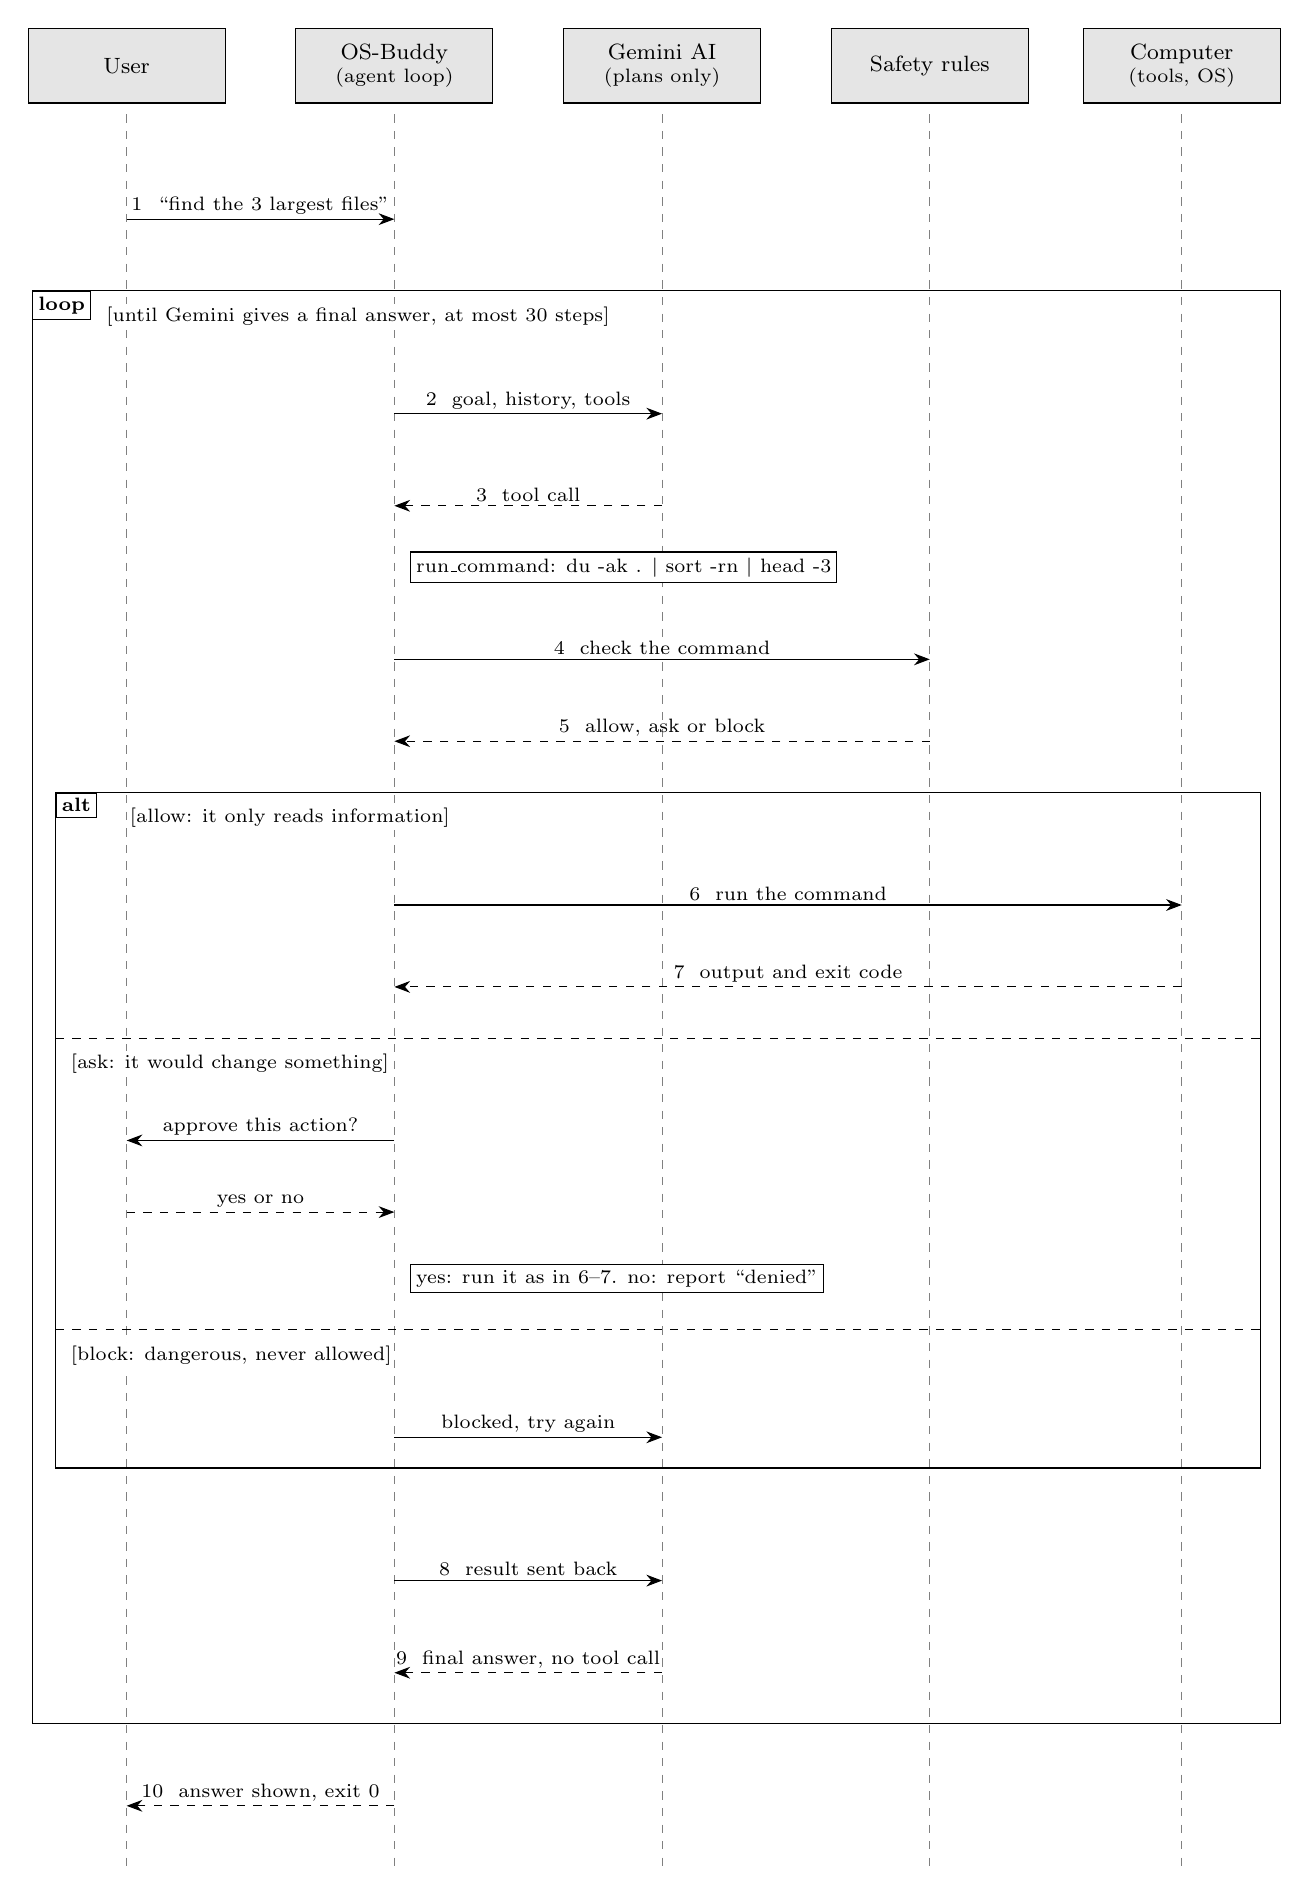
\begin{tikzpicture}[
  yscale=1.3,
  font=\footnotesize,
  part/.style={draw,fill=hdrgrey,align=center,minimum width=2.5cm,minimum height=0.95cm,inner sep=2pt},
  call/.style={-{Stealth[length=2mm]}},
  ret/.style={-{Stealth[length=2mm]},dashed},
  frame/.style={thin},
  tag/.style={anchor=north west,draw,fill=white,font=\scriptsize\bfseries,inner sep=2pt}]
\def\xU{1.3}\def\xA{4.7}\def\xG{8.1}\def\xP{11.5}\def\xC{14.7}\def\yEnd{-17.6}
\newcommand{\msg}[5]{\draw[#4] (#2,#1) -- (#3,#1)
  node[midway,above,font=\scriptsize,inner sep=1.5pt,align=center] {#5};}
% participants and lifelines
\node[part] at (\xU,0) {User};
\node[part] at (\xA,0) {\projectname\\[-1pt]\scriptsize(agent loop)};
\node[part] at (\xG,0) {Gemini AI\\[-1pt]\scriptsize(plans only)};
\node[part] at (\xP,0) {Safety rules};
\node[part] at (\xC,0) {Computer\\[-1pt]\scriptsize(tools, OS)};
\foreach \x in {\xU,\xA,\xG,\xP,\xC} {\draw[dashed,gray] (\x,-0.475) -- (\x,\yEnd);}
% 1 goal
\msg{-1.5}{\xU}{\xA}{call}{1~~``find the 3 largest files''}
% loop frame
\draw[frame] (0.1,-2.2) rectangle (15.95,-16.2);
\node[tag] at (0.1,-2.2) {loop};
\node[anchor=west,fill=white,font=\scriptsize,inner sep=1pt] at (1.0,-2.45) {[until Gemini gives a final answer, at most 30 steps]};
% 2-3 ask Gemini
\msg{-3.4}{\xA}{\xG}{call}{2~~goal, history, tools}
\msg{-4.3}{\xG}{\xA}{ret}{3~~tool call}
\node[draw,fill=white,font=\scriptsize,inner sep=2pt,anchor=west] at (\xA+0.2,-4.9)
  {run\_command: du -ak . \textbar\ sort -rn \textbar\ head -3};
% 4-5 safety
\msg{-5.8}{\xA}{\xP}{call}{4~~check the command}
\msg{-6.6}{\xP}{\xA}{ret}{5~~allow, ask or block}
% alt frame
\draw[frame] (0.4,-7.1) rectangle (15.7,-13.7);
\node[tag] at (0.4,-7.1) {alt};
\node[anchor=west,fill=white,font=\scriptsize,inner sep=1pt] at (1.3,-7.35) {[allow: it only reads information]};
\msg{-8.2}{\xA}{\xC}{call}{6~~run the command}
\msg{-9.0}{\xC}{\xA}{ret}{7~~output and exit code}
\draw[dashed] (0.4,-9.5) -- (15.7,-9.5);
\node[anchor=west,fill=white,font=\scriptsize,inner sep=1pt] at (0.55,-9.75) {[ask: it would change something]};
\msg{-10.5}{\xA}{\xU}{call}{approve this action?}
\msg{-11.2}{\xU}{\xA}{ret}{yes or no}
\node[draw,fill=white,font=\scriptsize,inner sep=2pt,anchor=west] at (\xA+0.2,-11.85)
  {yes: run it as in 6--7. no: report ``denied''};
\draw[dashed] (0.4,-12.35) -- (15.7,-12.35);
\node[anchor=west,fill=white,font=\scriptsize,inner sep=1pt] at (0.55,-12.6) {[block: dangerous, never allowed]};
\msg{-13.4}{\xA}{\xG}{call}{blocked, try again}
% 8 result back
\msg{-14.8}{\xA}{\xG}{call}{8~~result sent back}
% 9 final answer
\msg{-15.7}{\xG}{\xA}{ret}{9~~final answer, no tool call}
% 10 answer
\msg{-17.0}{\xA}{\xU}{ret}{10~~answer shown, exit 0}
\end{tikzpicture}}
\caption{Sequence diagram of one goal. Gemini only chooses actions; every action passes the safety
  rules before it reaches the computer, and each result goes back to Gemini until the goal is reached.}
\label{fig:sequence}
\vspace*{\fill}
\end{figure}

\clearpage
\section{Team Contributions}
The project will be done by a group of five. Each member will take one main area, so everyone
can work at the same time.

\begin{table}[H]
\centering
\caption{Division of work within the group.}
\label{tab:team}
\small
\begin{tabularx}{\linewidth}{@{}|R{3.3cm}|R{3.6cm}|Y|@{}}
\hline
\hdrrow \textbf{Member} & \textbf{Main area} & \textbf{What they will do} \\ \hline
\memB & Overall design and AI helper & Plan the design, build the main AI helper and the start of
  the program \\ \hline
\memC & Tools and admin scripts & Build the actions the helper can take and the admin scripts \\ \hline
\memE & Gemini connection & Connect to the Gemini AI and write its instructions \\ \hline
\memA & Safety rules & Write the safety rules and the approval questions \\ \hline
\memD & Testing and documents & Write the tests, set up automatic checks, and prepare the
  project documents \\ \hline
\multicolumn{3}{|l|}{\cellcolor{hdrgrey}\textbf{Shared by the whole group}} \\ \hline
\multicolumn{3}{|l|}{Planning, design decisions, checking each other's work, demonstration} \\ \hline
\end{tabularx}
\end{table}

\section*{References}
\begingroup\small
\begin{enumerate}\tightlist
  \item S.~Russell and P.~Norvig, \emph{Artificial Intelligence: A Modern Approach}, 4th ed., Pearson, 2020.
  \item Google AI for Developers, ``Gemini API documentation: Function calling,''
    \href{https://ai.google.dev/gemini-api/docs/function-calling}{https://ai.google.dev/gemini-api/docs/function-calling}.
  \item GNU Project, \emph{Bash Reference Manual},
    \href{https://www.gnu.org/software/bash/manual/}{https://www.gnu.org/software/bash/manual/}.
\end{enumerate}
\endgroup

\end{document}
